This project covers an exciting area of Computer Science with Machine Learning and Federated Learning.
I will be covering each in turn and also giving a more detailed analyses where it is deemed relevant to the project.
This project makes the following assumptions:

\begin{enumerate}
    \item The attacks that are carried out only interfere with the models, their parameters and their data. They do not involve network security based attacks or attacks that involve external agents in manners such as a Distributed Denial of Service (DDOS) attack.
    This is because these external agents are not unique to Federated Learning and have nothing to do with its process or how it is implemented.
    
    \item The Machine Learning Models' hyperparameters are optimal to the datasets we test on. Further, that we do not require additional fine tuning for it to achieve optimal performance in the context of a distributed system. Fine tuning the hyper-parameters of these models specifically is out of the scope for this project.
\end{enumerate}


\section{Machine Learning}

Machine Learning (ML) is a method of training models using sets of data to recognise patterns so that a trained model is capable of making predictions or decisions without explicitly being told what to do.\\ \\
The three main categories of ML are:
\begin{enumerate}
    \item Supervised Learning: the model is give the training data and a set of labels for what each piece of datum is. It is meant to learn from these data-label combos.
    
    \item Unsupervised Learning: the model has no labels and instead tries to find hidden patterns in the data.
    
    \item Reinforcement Learning: the agent tries to reach a certain goal and is given a score/reward depending on how well it achieves its goal.
\end{enumerate}
For the purposes of this project, we will only be focusing on Supervised Learning algorithms. For unsupervised learning it would become much more difficult to properly evaluate if the model is being tampered with. Human intervention is needed to check what hidden patterns the model is finding, which is not sustainable in this case.


\subsection{Neural Networks}
A Neural Network (NN) is a form of ML in which the ML model learns from its experiences with a given set of data. It achieves this through assigning weights to the connections between ``nodes" (like artificial neurons \cite{neurons}) in the network of the model. For models beyond 1 layer in depth, we also have the use of back-propagation (finding the gradient of the loss with respect to each of the weights) which makes it possible to apply efficient gradient descent for finding the optimal point. This is because these ML problems are often evaluated with a loss function where the purpose is to minimise the loss. A common loss function is Mean Squared Error (MSE) which minimises the average of squared difference between predictions and actual observations:
\begin{equation}
    MSE = \dfrac{1}{n} \Sigma (\hat{y} - y_i)^2
\end{equation}
An example of a basic NN is shown below where the thickness of each line represents the relative size of the weights for each connection.
\begin{figure}[htbp]
	\centering
    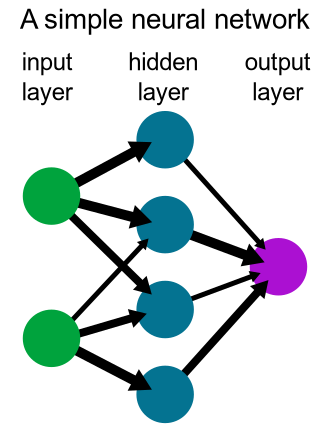
\includegraphics[scale=0.3]{background/neural_network.png}
	\caption{Neural Network image from Wikipedia, the free Encyclopedia}
	\label{fig:nn}
\end{figure}

\subsection{Deep Learning}
Deep Learning (DL) is a subset of Machine Learning that focuses on NNs with many layers. A conventional NN would only have 1 hidden layer whereas a DL network could go into the 10s or 100s (or more!). This is to accommodate ever-increasing dataset sizes. In the modern age, the sheer increase in data and parameters associated with ML is getting so large that certain problems require DL networks to solve them. This is so that every minute feature and detail can be extracted from the datasets and be properly represented by the model \cite{deeplearningbook}.\\ \\
They also include the use of activation functions between the layers. An activation function creates an output based on the output of the previous layer by applying a non-linear function to change it. Some of the most common to use are the $\tanh$ function and Rectified Linear Unit (ReLU \cite{relu}). We show some examples in \ref{tbl:activation-tbl}. \\ \\
For constructing DL models we will need to use some combination of these activation functions (and potentially others not mentioned \cite{wiki:activation}).

\newcommand{\tanhFunc}{
    $\tanh(x) = \dfrac{e^x - e^{-x}}{e^x + e^{-x}}$
}
\newcommand{\ReluFunc}{
    $ReLU(x) =
    \begin{cases}
      0 \hspace{0.5cm} $if $ x \leq 0\\    
      x \hspace{0.5cm} $if $ x > 0
    \end{cases}
    $
}
\newcommand{\SigmoidFunc}{
    $\sigma(x) = \dfrac{1}{1 + e^{-x}}$
}

\newcommand{\tanhDerivative}{
    $1 - \tanh(x)^2$
}
\newcommand{\ReluDerivative}{
    $
    \begin{cases}
      0 \hspace{0.5cm} $if $ x < 0\\
      1 \hspace{0.5cm} $if $ x > 0\\
      undefined \hspace{0.5cm} $if $ x == 0
    \end{cases}
    $
}
\newcommand{\SigmoidDerivative}{
    $\sigma(x)(1 - \sigma(x))$
}

\pgfplotsset{width=3.3cm,compat=1.9}
\newcommand{\sigmoidGraph}{
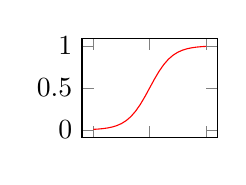
\begin{tikzpicture}
    \begin{axis}[xticklabels={,,}]
    \addplot[color=red]{1/(1 + exp(-x)};
    \end{axis}
\end{tikzpicture}
}
\newcommand{\tanhGraph}{
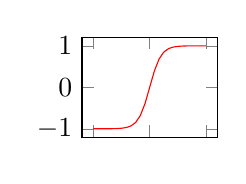
\begin{tikzpicture}
    \begin{axis}[xticklabels={,,}]
    \addplot[color=red]{(exp(x) - exp(-x))/(exp(x) + exp(-x))};
    \end{axis}
\end{tikzpicture}
}
\newcommand{\reluGraph}{
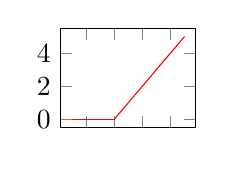
\begin{tikzpicture}
    \begin{axis}[
        domain=-3:5,
        xticklabels={,,},
        ]
        \addplot+[mark=none,red,domain=-3:0] {0};
        \addplot+[mark=none,red,domain=0:5] {x};
    \end{axis}
\end{tikzpicture}
}

\begin{center}
    \begin{longtable}{ | m{3.5em} | m{12.3em} | m{10.9em} | m{5.6em} | }
    \caption{Activation Function Table}
    \label{tbl:activation-tbl}
    \hline
    \textbf{Name} & \textbf{Function} & \textbf{Derivative} & \textbf{Example} \ \\ \hline
    tanh & \tanhFunc & \tanhDerivative & \tanhGraph \ \\ \hline
    ReLU & \ReluFunc & \ReluDerivative & \reluGraph \ \\ \hline
    Sigmoid & \SigmoidFunc & \SigmoidDerivative & \sigmoidGraph \ \\ \hline
    \end{longtable}
\end{center}

How these activation functions are used and when they are used can have an effect on the performance of a NN. Even fine-tuning certain combinations of activation functions can greatly improve performance \cite{activation_combined}.

\subsection{Convolutional Neural Networks}
DL models can be used for a variety of tasks but one that is quite common is that of image recognition. The popular structure for specific types of DL networks that focus on this is that of Convolutional Neural Networks (CNN). While typical NNs struggle in the complexity and detail of images, CNNs are more able to ``successfully capture the Spatial and Temporal dependencies in an image through the application of relevant filters" \cite{eli5_convnet}. The number of layers could in theory be increased but that adds vast computational power and it could lead to the over-fitting of the network. \\ \\
Instead we go for different architecture that consists of three distinct types of layers \cite{convnet}:
\begin{enumerate}
    \item \textbf{Convolutional Layer:} this layer takes a predefined kernel \cite{kernel} and applies it to the 2D image. If the input has more than one channel (e.g. an RGB image), then it is applied to each channel. The kernel that is used can change which features are highlighted and extracted depending on the use case. Some common kernels in Computer Vision are blurring kernels and Sobel kernels.The size of the kernel and how much it strides by in each step can decide as to how much reduction in dimensions there are.
    
    \item \textbf{Pooling Layer:} this layer is used to help decrease the spatial size of the previously convolved feature. This can then in turn decreases the processing power required to process the data as the size of the dimensions can be greatly reduced. This can be quite destructive to the data and so 2 more common approaches are to use a 2x2 kernel with a stride of 2 or to use a 3x3 kernel with a stride of two. The latter allows for overlap of the pixels but a kernel size above 3x3 can result in greatly decreased performance. Pooling is used to help detect patterns in images that are usually far too big for smaller kernels to detect actual patterns.
    
    \item \textbf{Fully-Connected Layer:} this acts like a typical NN and will try and form scores for the relevant classes/predictions based while connected in the standard way of being connected to all the neurons of the previous layer.
\end{enumerate}
An example of how these layers come together and form a CNN is below:
\begin{figure}[htbp]
	\centering
    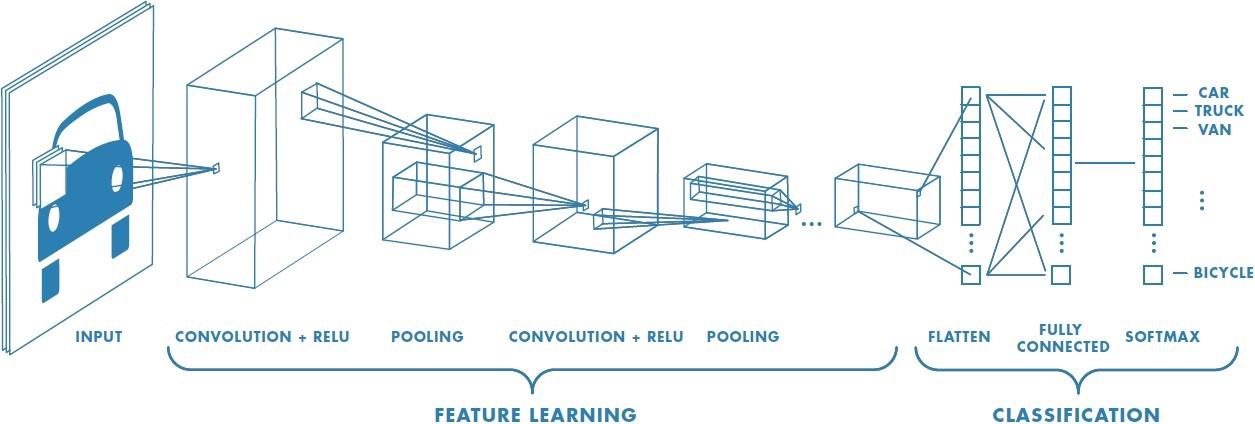
\includegraphics[scale=0.3]{background/cnn_example.jpeg}
    \caption{Visual Representation of CNN Layers \cite{eli5_convnet}}
    \label{fig:cnn-layers}
\end{figure}

For simple datasets like MNIST (where the dimensions of the images is only 28x28 and the image itself is fairly basic) we don't need a particularly complex NN beyond having the initial layer contain 784 (28x28) weights and so it doesn't necessarily benefit from a CNN. For something like the MedMNIST datasets, they are not in a higher dimension but are of higher complexity than that of standard MNIST and so more greatly benefit from the use of a CNN. Other examples of datasets that benefit this way are FashionMNIST \cite{fashion} and CIFAR-10 \cite{cifar}.\\ \\
One difference to note about the initial layer of a CNN compared to a standard NN is that it remains represented as a 2D array instead of being streamed into a 1D vector. This is something that allows the network to help recognise the patterns better as it retains the structure of the original image more precisely.



\section{Privacy Preserving Techniques}

With various methods of ML being applied to all manner of things to try and help make predictions about life better, it is only natural that the data in question will include personal data. Whether this is through monitoring app/website usage or very simply tracking what people ``like" or send to each other, the data is personal to each user and as such the experience of each user is personal. \\ \\
However, data can stray beyond this into more truly personal information such as that of the medical nature.
This is trickier to deal with, given that medical data is very tightly controlled and restricted due to its highly sensitive nature and the governing bodies controlling it are usually very unwilling to share. 
Now in the past this wasn't really an issue as typically only medical professionals of the governing organisation (e.g. the National Health Service (NHS)) would want access to this data and actually have any good reason. 
So it was very easy and efficient to deny any external access. 
However, we now live in a world where the prevalence of ML has made external researchers' access to data increasingly valuable to society. 
Users, beyond medical professionals, want access to this highly sensitive data to try and make the world a better place.
\\ \\
Whether this is in trying to train a model to recognise cancerous cells or early onset dementia, data surrounding that is needed to accurately make these predictions. 
So, to be able to push the field of medicine forward and to leverage to full power of modern day computing, we as software engineers need access to this data. 
So several methods of trying to preserve the privacy of the users of this data have been created to tackle this.

\subsection{Homomorphic Encryption}
Encrypting data seems to be a fairly intuitive starting point for trying to keep the privacy of user's data secured. 
For cloud computing \cite{cloud_fhe}, it is almost a necessity that the data is encrypted in some manner as otherwise employees of the company potentially have access to this data and could act maliciously \cite{access_private}. 
However, it results in a system where no one can read or understand the data without the appropriate decryption keys (usually not stored on a centralised server) and so trying to perform any calculations or processing on the data is somewhat redundant. 
So in comes the idea of Homomorphic Encryption. This is a style of encrypting data such that you are able to perform some given calculation on the encrypted data without the need for decrypting it first (e.g. addition).
\\ \\ 
However, only being able to perform 1 operation on the data isn't particularly useful and so the more impressive standard of Fully Homomorphic Encryption (FHE) was postulated \cite{fhe}. 
In theory, FHE allows for any number of operations to be performed (although current operations are typically just addition and multiplication) on the encrypted data. 
However, it is not a simple/intuitive system to implement for any given task and so for certain tasks, it may not be an ideal method on preserving the privacy of data.


\subsection{K-Anonymisation}
The idea behind anonymising data is to not be able to associate an individual person's data record with their actual identity in a given dataset. 
This helps to reassure that the data will not cause any worry or harm to that individual. This has the added side-effect of no longer making the data personal anymore and so more freely able to be used beyond the governing owner of that data. 
This is hugely beneficial to both parties and is a great starting point for preserving the privacy of the data. 
\\ \\
However, this is not as simple as it sounds and many attempts to pseudo-anonymise the data have resulted in people able to use more than one available dataset to link medical data with more available (and less sensitive) data like a voter list \cite{failed_anonymisation}.
\\ \\
Even if that weren't the case, you get certain attributes that when taken together are potentially able to identify a person. These are called quasi-identifiers. 
An example would be if you knew their post code and their date-of-birth, you could potentially figure out a disease they have if no one in that postcode shares that date-of-birth with them. e.g. id=3 in Table \ref{tbl:pre-anon}.
\\ \\
A way to tackle these is through the use of k-anonymising the data. A table of data is k-anonymous if every record in the table is indistinguishable from at least k-1 other records, with respect to every set of quasi-identifiers (not something that is itself a unique identifier, but when paired with other quasi-identifiers it can identify someone). 
The 2 styles of doing this are perturbative methods and non-perturbative methods but seeing as perturbative methods (e.g. adding noise) does not retain data integrity, we won't be considering it. 
Two main ways of achieving k-anonymity for non-perturbative methods are generalising the data (replacing attribute values with something more generalised e.g. 54321 $\longrightarrow$ 54***) and suppression (deletion of row or column e.g. row with id=3 in Table \ref{tbl:pre-anon}).
\begin{center}
    \begin{longtable}{ |c|c|c|c|c| }
    \caption{Pre-Anonymisation}
    \label{tbl:pre-anon}
    \hline
    \textbf{id} & \textbf{sex} & \textbf{DoB} & \textbf{postcode} & \textbf{disease} \ \\ \hline
    1 & female & 1998-03-13 & SW7 2BU & anxiety \ \\ \hline
    2 & female & 1998-10-27 & NW1 9LJ & anxiety \ \\ \hline
    3 & female & 1997-01-22 & AL9 7TA & chicken pox \ \\ \hline
    4 & male & 1999-11-11 & HP11 1UA & ADD \ \\ \hline
    5 & male & 1999-06-18 & HP14 4JQ & Dyspraxia \ \\ \hline
    6 & male & 1999-06-21 & HP11 2DQ & ADHD \ \\ \hline
    \end{longtable}
    
    \begin{longtable}{ |c|c|c|c|c| }
    \caption{2-Anonymised}
    \label{tbl:2-anon}
    \hline
    \textbf{id} & \textbf{sex} & \textbf{DoB} & \textbf{postcode} & \textbf{disease} \ \\ \hline
    \rowcolor{lightgray} 1 & female & 1998 & London & anxiety \ \\ \hline
    \rowcolor{lightgray} 2 & female & 1998 & London & anxiety \ \\ \hline
    \rowcolor{gray} 4 & male & 1999 & High Wycombe & ADD \ \\ \hline
    \rowcolor{gray} 5 & male & 1999 & High Wycombe & Dyspraxia \ \\ \hline
    \rowcolor{gray} 6 & male & 1999 & High Wycombe & ADHD \ \\ \hline
    \end{longtable}
\end{center}

The data is still susceptible to homogeneity and semantic attacks [Table \ref{tbl:2-anon}] and while {l-Diversity} can fix the former there is never any guarantee that a dataset is 100\% completely and truly anonymised. With k-anonymisation, a specific data record can't be identified with any given individual but information can still be inferred. The governing body behind the data sometimes has to make a decision about what is an acceptable level of anonymisation without completely destroying any utility or functionality behind it. There are some techniques being investigated through clustering of the data to help minimise information loss \cite{anon_cluster} but again, these only go so far. It should also be noted that k-anonymity can only work on table and record style data instead of things like images and so has its limitations there.


\subsection{Secure Multi-Party Computation}
A different approach for preserving privacy is when you have multiple parties all wanting to calculate something based on each others' data but no one wants to share their data. For this we have Secure Multi-Party Computation (MPC) and it is when 2 or more parties share their data with a 3rd trusted party and it carries out an algorithm that doesn't reveal anything about the parties' data that was given (unless the result of the function revealed the values anyway). \\ \\
However this involves a trusted 3rd party and so a different style would be through something called Secret Sharing (SS) and will be explained through the BGW Protocol \cite{bgw}. This expresses the function that is computed as an arithmetic circuit containing addition and multiplication gates. It involves the parties splitting up their value into ``shares" and sending them off to the other parties. Each party then calculates the function on those shares, broadcasts the output as new shares before combining the shares it receives into a value. This is shown in Figure \ref{fig:bgw}.
\begin{figure}[htbp]
	\centering
    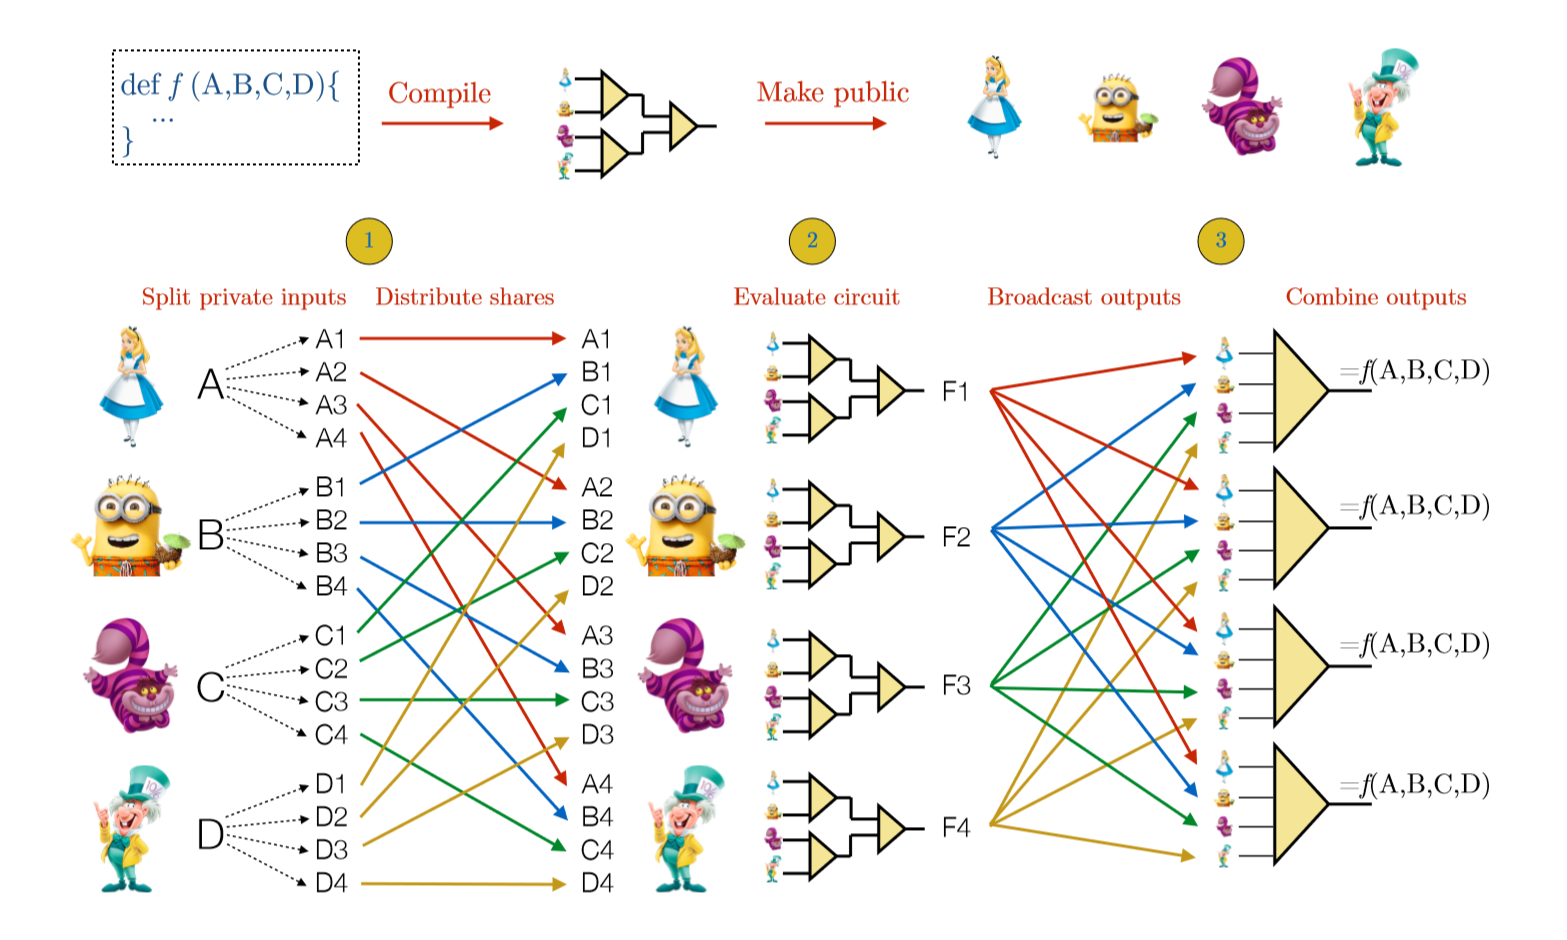
\includegraphics[scale=0.3]{background/bgw.png}
	\caption{BGW Protocol, courtesy of N. Dulay's Privacy Engineering Slides \cite{priv_eng}}
	\label{fig:bgw}
\end{figure}


\subsection{Differential Privacy}
Another method for preserving privacy is Differential Privacy (DP). DP guarantees that when you query a dataset D, the result that you get will be approximately the same (if not the same) irrespective of the presence of whether or not the dataset contained a certain value. This can be summarised as:
\begin{equation}
    Pr[x | y \in D] \approx Pr[x | y \notin D]
\end{equation}
As we want = instead of $\approx$ without destroying utility, we have the difference shown with $\epsilon$ such that:
\begin{equation}
    Pr[M(D) = y] \leq e^\epsilon Pr[M(D') = y]
\end{equation}
Where D is the dataset with no changes and D' is the dataset with the missing row. M is the function applied to D that computes the output and ensures privacy. We have to make sure that the two datasets satisfy the condition that they are neighbouring, i.e. they differ by exactly one row. This is what it means for a mechanism to be $\epsilon$-Differentially private. \\ \\
For achieving DP, the key ingredient is adding noise to the data until the above requirement is satisfied. This can be done with either Gaussian or Laplacian noise, with Laplace noise being the more common choice for DP. Typically, you draw from a Laplacian distribution that is $L(1/\epsilon)$ for the mechanism to remain $\epsilon$-Differentially private. Laplace's probability density function (pdf) is defined as:
\begin{equation}
    L(x|\mu,b) = \dfrac{1}{2b} \exp \left( -\dfrac{|x - \mu|}{b}\right)
\end{equation}

For ML models, depending on where we add the noise to, our mechanism will either be Locally or Globally differentially private. If the noise is added to the inputs of the model then it is Local DP. This involves each client adding noise so as to help protect their data. This helps ensure that each user has plausible deniability as you could never accurately claim that a certain client's specific data is of some specific value. If the noise is added to the end then it is Global DP. This is more desirable if the owner of the person taking the data and training with it is trustworthy as you can normally achieve more accurate results \cite{global_dp} as the input data has not been modified or changed. \\ \\
Interestingly, there are cases where adding noise to the gradient of models in very deep NNs \cite{dnn_noise} or as a form of regularisation for data augmentation \cite{robust_corrupt_noise} can help improve the generalisation performance of the trained model through either greater feature extraction ability or from reducing over-fitting.


\section{Federated Learning}

If data stayed amongst those that owned or governed it, then there would be less of a need for privacy preserving mechanisms. 
However in FL, while clients do process data on their own devices, the results are then sent to a centralised server for aggregation. 
\\ \\
In FL we are trying to have all the clients keep hold of their data whilst still being able to contribute it in a form that does not actually involve the sharing of it. The data is usually uneven as each client involved could have wildly different sizes of data or even wildly different backgrounds for the data. Two examples of this would be:
\begin{enumerate}
    \item Monitoring users' interactions with an app and training a model on the user's phone to make accurate predictions about what ads they'll like. 
    The model update calculated will be hyper-specific and over-fitted to an individual user at first. 
    But when you get 10s of 100s of users' models all being sent to a centralised server for aggregation, the model that will be sent back to each user will be much more generalised and better at making more accurate/clever predictions. 
    Through more rounds of back and forth it will eventually converge.
    
    \item If you had a group of hospitals that all had a large amount of patient data and they wanted to train a model for some arbitrary reason, they would be able to again train locally and send off the model just like before. 
    However, you could end up having 1 hospital that deals with a disproportionately large amount of elderly patients and their model would be skewed in that favour. 
    This can help the other hospitals who do not have as much access to such data. 
    This is a mutually beneficial exchange, as it also gives the original hospital more access to younger patient data. 
    As such, results are more easily able to generalise regardless of the age.
\end{enumerate}
As you can see, through FL, we are able to get more accurately trained models on otherwise private and sensitive data. 
This provides unprecedented potential for medical data to be used for research purposes where we will not need direct access to the data. However, as too-good-to-be-true as this might sound, there are obvious barriers in the way. 
For the hospitals and practices, not only will they have to standardise all of their data in an agreed-upon way, they will also have to hugely invest in some form of computing infrastructure such as something on-premise or in the cloud \cite{future_health_fl}. 
This involves a high initial cost as there is computing power needed for training such large amounts of data. 
This also does not mean that researchers outside of the hospital will even be able to use the data anyway, just that the Clinicians, Patients, Manufacturers and Healthcare providers can all benefit from the improvement of the ML-based systems \cite{future_health_fl}.

\subsection{Training}
The process of training the data for FL is as follows and is shown graphically in Figure \ref{fig:federated_learning}:
\begin{enumerate}
    \item Clients retrieve model from the central server.
    
    \item Each Client trains the model on its data and calculates a model update.
    
    \item Clients send the updates to the central server.
    
    \item Central server aggregates these updates together.
    
    \item Central server sends the new shared model back to the clients.
    
    \item Repeat 1-5 until convergence.
\end{enumerate}
\begin{figure}[htbp]
	\centering
    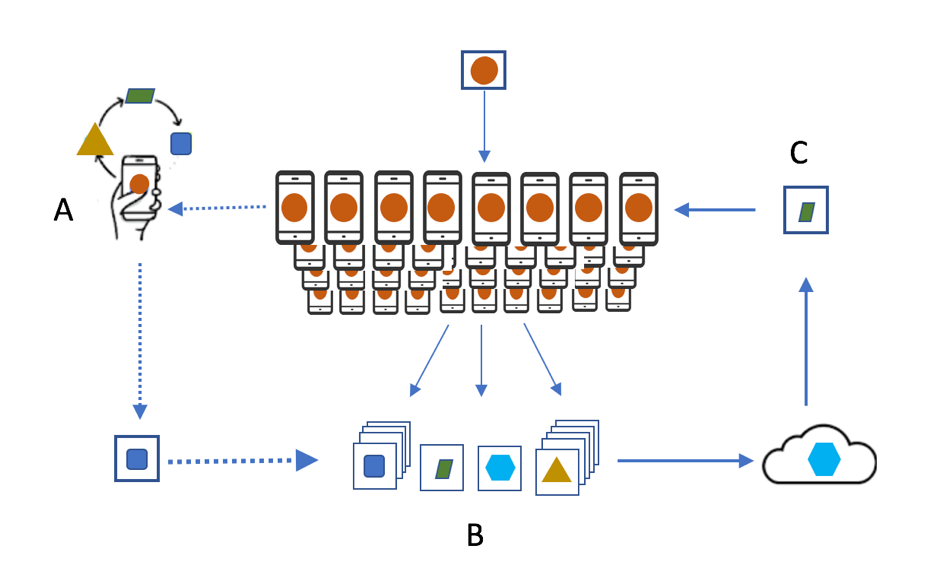
\includegraphics[scale=0.3]{background/federated_learning.png}
	\caption{Rough example of the exchange of ML models on user devices \cite{federated_learning}}
	\label{fig:federated_learning}
\end{figure}
The process by which the aggregation could be done is usually one of Federated Stochastic Gradient Descent (FedSGD) \cite{fedsgd} or Federated Averaging (FedAvg) \cite{fedavg}.
FedSGD aggregates on the models' gradients whereas FedAvg aggregates on the models' weights/parameters. \\ \\
In comparison to a baseline model with no FL employed, close to the exact same results can be achieved with standard FL with between a 0.008 and 0.014 Area under the Curve (AUC) difference \cite{babu}.


\subsection{Personalised Federated Learning}
Through this typical process of training, every client receives the same global model that has been aggregated through a contribution from everyone in some way, shape or form.
However, this might end up not being the most ideal strategy for achieving the best accuracy globally and locally.
Especially when it comes to non-independent and identically distributed (iid) data, being able to adapt the models that are sent out could be crucial for getting good performance.
\\ \\
One style in which this can be done is with Federated First Order Model Optimisation (FedFomo) \cite{fedfomo}.
Here, the method involves each client having a goal that it aims for that is based on its own validation and test data.
The central server then tries to group clients that want to achieve similar goals together so that they can contribute towards their own model together.
\\ \\
This method is a tad odd in that it does not seem to focus on generalisation and making sure the models utilise all of the data from the clients in a constructive way.
However, there are a variety of different ways in which this personalisation could be implemented and ultimately the solution chosen should reflect the problem that is trying to be solved.


\subsection{Privacy Amplification}
Attempting to amplify privacy via user sampling is a method in which not all clients are chosen to participate at every federated round.
Its main use is for helping to preserve the privacy of the clients involved through minimising honest-but-curious clients' interest in information leakage.
\\ \\
This seems like it would be an interesting solution to help the clients' privacy but unfortunately it is not without its drawbacks.
Experiments have shown that generally decreasing the probability (p) for clients to be picked leads to quite a significant decrease in convergence rate as well as a decrease in training accuracy \cite{privamp}.
\\ \\
Depending on what trade-offs you are willing to make, its gives the user quite a bit of flexibility in terms of having either more privacy, better accuracy or some combination of both.



\subsection{Possible Attacks}
Aggregating on the model updates from distributed clients seems to be a great strategy for accessing private data without it being leaked out. 
However, as all things that involve a human element, it can be exploited. 
The two main types of attacks are targeted and untargeted attacks.
Targeted attacks focus on the attacker trying to get the model to predict a specific thing incorrectly, e.g. telling an MNIST dataset that 5 is actually 7 to the extent that the global model starts classifying it as such. 
Untargeted attacks are just when the attacker tries to get the model to not reach convergence or a good accuracy.
\\ \\
Some different styles of poisoning (changing something in a negative manner) are highlighted in Table \ref{tbl:poisoning}. 
All methods excluding the final option are easily accessible to any client.
This is because the client owns their data and as such is in full control and can change it as needed. 
In terms of model reading and writing, the client will receive the model and can send back whatever they like. 
The central server has no way of stopping any of this and without breaking the whole notion behind federated learning, cannot have the clients data checked for tampering (unless some encrypted form of ML was used, which is extremely slow and computationally expensive). \\ \\
In theory if you had control of the client side as well (e.g. a mobile app), then you probably would not need to worry about the model poisoning side of things. 
The final option assumes that the malicious client essentially has complete control over the system and at this point it is essentially impossible to design a robust aggregation system \cite{robagg_fl}.
\begin{center}
    \begin{longtable}{ |c|c|c|c|c| }
    \caption{Poisoning Attacks \& Corruption Examples \cite{robagg_fl} - \textbf{Data Write} is changing of data in dataset, \textbf{Model Read} executing code based on model update before update takes place, \textbf{Model Write} is running code instead of standard update code and \textbf{Aggregation} is running code instead of the standard aggregation function on the central server}
    \label{tbl:poisoning}
    \hline
    \textbf{Corruption Type} & \textbf{Data Write} & \textbf{Model Read} & \textbf{Model Write} & \textbf{Aggregation} \ \\ \hline
    None & - & - & - & - \ \\ \hline
    Static Data Poisoning & Yes & - & - & - \ \\ \hline
    Adaptive Data Poisoning & Yes & Yes & - & - \ \\ \hline
    Update Poisoning & Yes & Yes & Yes & - \ \\ \hline
    Byzantine & Yes & Yes & Yes & Yes \ \\ \hline
    \end{longtable}
\end{center}
There's also the case to handle where it may look like an attacker is trying to cause damage when it actuality it's just a faulty client. 
Depending on the level of damage done it may be beneficial to actually not block faulty clients, as they may introduce noise that improves the model's generalisability \cite{dnn_noise, robust_corrupt_noise}. 
However, you are most likely going to end up blocking them as they could be damaging your performance without themselves realising it.

\subsubsection{Data Poisoning}
This involves maliciously changing the data in an attack. 
It could be done by adding noise or changing labels but as long as the original dataset has been changed, it is considered as having undergone a data poisoning attack. 
It has been shown that data poisoning attacks have been able to achieve a high-confidence of misclassification for deep NN \cite{poison_dnn}. 
\\ \\
There is also a difference between static and adaptive data poisoning. 
Static is where the data is poisoned once at the beginning (prior to training). 
Adaptive is seeing how the models change and then change the data at the beginning of each round so as to accommodate for it. 
Adaptive is more complex but could have the potential to achieve better results as the attack ends up being more tailored.

\subsubsection{Model Poisoning}
This technique uses the model to help craft a specially designed model update. 
In the targeted case, we would have a goal for misclassification but with all of the other users averaging out the poisoning, we would need to change the update in such a way as to negate the combined effects of the benign clients.
Evaluation done has shown that this can lead to 100\% confidence in target misclassification while also impressively achieving convergence of the model \cite{adversarial_lens}. 
\\ \\
To help avoid detection (if the aggregation done is attempting to be robust) where the central server has stealth metrics to identify malicious clients, the malicious objective can be modified so as to account for these detections. 
With this you can normally go undetected for the majority of the rounds but a more clever strategy where we use ``alternating minimisation" to account for both stealth and model poisoning so as to help go undetected for all of the rounds \cite{adversarial_lens}. 
The aim is to minimise for the adversarial objective first and then minimise for the stealth objective for any given epoch.

\subsubsection{Free-Riding}
Attacks do not necessarily come in the form of trying to manipulate the model in a negative way. 
One method involves ``Free-Riding" \cite{free_riding} where the client instead has a goal of trying to gain the completed model without actually contributing anything to the cumulative effort. 
This might be done when the models have commercial/intellectual value and can subsequently lead to intellectual property/financial loss. 
The client would have to trick the rest of the clients into thinking that they have useful and valuable data to contribute.
The size at which the free-rider decides to claim their data is up to them, but is typically the average of the rest of the data.
\\ \\
The initial way of doing this would be to simply return the model's parameters at each round. 
However, this can easily be checked for by the central server.
The way to get around this is to add some Gaussian white noise to the parameters and gradients that is of a similar structure to the benign clients' responses.
This is done by monitoring the mean and variance of the other responses and adjusting accordingly at each round.
The main effect adding noise has is that the resulting variance of the accuracy will increase and the amount it increases is dependant on the variance used by the free-rider.
However, it should be noted that the increase in variance did not appear to show a significant increase in loss and so it could be considered worth it for the anonymity.
\\ \\
However, the noise variation that is typically observed by the benign clients, through something like SGD, decreases as the model converges.
So the free-rider must in turn decrease their noise in a similar asymptotic manner to their noise added.
This again works until a certain extent but anomaly detection methods such as Deep Autoencoding Gaussian Mixture Models (DAGMM) \cite{dagmm} have been shown to detect the free-riders as anomalies \cite{freerider_defence}.
\\ \\
The main way for free-riding clients to then hide is to use a ``delta-weight attack" \cite{freerider_defence}.
Here, they instead use the difference between the previous and current global models and assign that difference to the gradient weights of the parameters.
This emulates the average gradient weights from all of the other clients and so becomes a very neutral client and so can avoid detection much better.
Wonderfully, with the use of privacy amplification, it becomes easier for the central server to detect these delta-weight attacks.
This is because they are only getting model updates every few rounds when selected and so their model that they contribute has gradients with far more eccentric changes than they would otherwise have.
\\ \\
``This result is in agreement with our theory, for which the convergence speed is inversely proportional to the relative size of the free-riders" \cite{free_riding}. 
However, it should be noted that too many free-riders will detriment the global model to some extent and so these attackers should be wary of the effect that they have.
This becomes slightly less of a problem with DP as the inherent added noise almost mimics that of a free-rider and so there is more expectation of fluctuations of accuracy.
It also allows the free-riders to hide themselves better amongst the other clients, which is a nice added bonus for them.
\\ \\
The nature of free-riding becomes quite an elusive game of cat-and-mouse with ever increasing concealing and detection.
It's quite a wondrous area for further investigation and implementation testing.





\section{Non-Robust Aggregation}

When it comes to aggregation, there are a variety of different methods which people have tried so as to achieve different results.
This can vary from using encrypted data, simple weighted-averaging of data or more robust methods.
When it comes to non-robust strategies, the typical focus is on trying to make the accuracy as good as possible and ideally with non-iid data.


\subsection{FedSGD}
FedSGD is based on the idea that you would sample the gradients of the model from each client and then have them all averaged proportionally based on the number of samples of each client.
The update strategy is simply that of SGD:
\begin{equation}
    \omega_j = \omega_j - \alpha \dfrac{\delta E_i}{\delta \omega_j}
\end{equation}
Where E is the error function (typically $L^2$ norm or cross-entropy) and w is the parameter that's being updated.
\\ \\
It sometimes also involves a selective parameter update, where only a certain number of the parameters are chosen each round.
This can be done at random but a smarter way is to use the models that have the largest gradient change and so in theory will contribute the most to the global model.


\subsection{FedAvg}
FedAvg was made to improve on FedSGD by instead focusing on the model weights instead of the model gradients \cite[section 2.1]{robagg_health}.
This has been shown to be an improvement on using the gradients and is typically used in other modern aggregation tasks.
It can be described through the formula:
\begin{equation}
    \theta_g = \mathlarger{\mathlarger{\sum}}_{i=0}^{\infty} \dfrac{d_i}{d} \theta_i
\end{equation}
Where $d$ denotes the entire dataset size, $d_i$ is the size of the dataset for model i and theta is the model parameter.


\subsection{Federated Matched Averaging}
Federated Matched Averaging (FedMA) \cite{fedma} was brought about to solve federated learning accuracy problems that occur in modern architectures and models such as LSTMs and CNNs.
Due to their deep and more complex nature, these architectures do not aggregate well under more coordinated style aggregations, like those found in FedAvg.
\\ \\
The algorithm works by aggregating the models layer-by-layer by starting with the initial layer and performing a weighted-averaging on it.
It then proceeds to broadcast this layer out to the clients and the clients then continue to train all of the layers after the broadcasted layer for a few rounds.
The aggregation then happens for the second layer and the process is repeated until the last layer.
Now, the number of times communication is required is equivalent to the number of layers and not a more arbitrary hyper-parameter set by the central server.
In theory, FedMA is then supposed to have far fewer number of communication rounds compared to FedAvg while out-performing it.
Experiments show \cite{fedma} that FedMA is capable of out-performing all other aggregation methods in accuracy across a variety of datasets that use more complex architectures.


\subsection{Auto-FedAvg}
Auto-FedAvg \cite{autofa} was born out of the need to handle non-iid data, whilst still improving overall accuracy.
Instead of having the weights for the weighted-averaging of the aggregation be fixed, they become learnable parameters that can adapt as the aggregation rounds occur.
\\ \\
In this algorithm there are two sets of weights: $\alpha$ and $\beta$.
$\alpha$ contains the set of learnable weights that the central server uses for aggregation and $\beta$ is what $\alpha$ is parameterised by during the learning process through an activation function $\gamma$.
In this case $\gamma$ can either be the Softmax function or a Dirichlet distribution where $\alpha$ is the set of random variables with concentration $\beta$. 
Dirichlet is as follows:
\begin{equation}
    Dir(\alpha | \beta) = \dfrac{1}{B(\beta)} \mathlarger{\mathlarger{\prod}}_{k=1}^{K} \alpha_k^{\beta_k-1}
\end{equation}
where $B(\beta) = \frac{\prod_{k=1}^K \Gamma(\beta_k)}{\Gamma (\sum_{k=1}^K \beta_k)}$ and $\Gamma(z) = \Sigma_0^\infty x^{z-1} e^{-x} dx$ is the gamma function.
\\ \\
Each round, the clients sample a mini-batch of their data and compute the $\alpha$ before using these weights in the aggregation.
The loss of the $\beta$ weights is then calculated with regards to the mini-batched data before $\beta$ is subsequently updated with $\gamma$.
The server then gathers up each $\beta$ weights from each client's local loss calculation and they are averaged to form the $\beta$ for the next round that is used to calculate the $\alpha$.
\\ \\
\textit{N.B. the paper relating to this method \cite{autofa} was released in April of 2021 and is still under development. As such, the methodology and implementation is still up to change as well as their experimentation results. In this area, it claims to be SotA and that it is better than FedMA in similar tasks, but this has not been peer-reviewed as of writing.}


\section{Robust Aggregation}

Unfortunately, having a raw aggregation method is suspect to a variety of potential attacks from any number of malicious users. 
In some cases, it might take a single client to have the model predict inaccurately. 
As such, we have to look outside non-robust aggregation methods like FedSGD and FedAvg. 
This can typically involve not including the malicious clients in the aggregation, giving the malicious clients a lower weighting in the aggregation and/or just completely blocking the clients once a certain threshold is met. 
\\ \\
Any of these methods have their cons in that it is possible in all cases to end up blocking at least one of the benign clients as well. 
When the number of clients is small this can have a much more detrimental affect due to a significant chunk of the training data is lost. 
Increasing the number of clients would mitigate the effect of this but there is still an issue of have the benign clients' data lost. 
A couple of different methods for robust aggregation will be introduced along with their performance under different styles of attacks.

\subsection{Krum}
To tolerate $f$ byzantine clients (malicious/faulty) out of a total of $n$ clients, Krum \cite{krum} achieves its byzantine-resilience property by looking at every subset of $n-f-1$ clients. 
It goes through each client and calculates the sum of the squared-distances between the client and their closest $n-f-2$ neighbours.
This becomes the score of that client and Krum takes the client with the best score and uses a data sample from that client.
With this method, Krum is able to theoretically tolerate up to f byzantine clients under the condition of $2f + 2 < n$. 
\\ \\
Another development on Krum brings in the idea of averaging to it, called Multi-Krum (MKRUM).
You take the top scoring $n-f$ clients' parameter vectors and average them together so as to be able to better leverage multiple correct (or at least correct by KRUM standards) clients.
This helps to reduce waste and not to throw away data. However, MKRUM still (and even more so Krum) throws away a lot of clients' data that might be useful. It also takes on a position where $f$ might not be chosen correctly, leading to even more data unnecessarily being thrown away.

\subsection{Coordinate-wise Median}
A simpler approach to choosing an individual client's parameters is through Coordinate-wise Median (COMED) \cite{comed}.
For all parameter vectors from all of the clients, COMED takes the median value of each of the parameters throughout all of the models.
This is defined mathematically as:
\begin{equation}
    g_k = med\{x_k^i: i \in [m]\}
\end{equation}
where k is the k-th parameter and m is the number of clients involved.
This very nicely gets to utilise all of the clients to try to have as balanced of a choice as possible for all of the model parameters.
It also performs quite well, generally better than MKRUM in an adversarial test while being a bit more sensitive to noise without any bad clients involved \cite{robagg_health}.

\subsection{Adaptive Federated Averaging}
A different way to handle byzantine clients is to simply block them, as done by Adaptive Federated Averaging (AFA) \cite{afa}.
It determines if a client is malicious based on the cosine similarity ($s_k$) between the model updates from the clients and the global aggregated model's parameters.
With this it also adaptively assigns weights to the clients for aggregation.
\\ \\
Assuming that the number of byzantine clients is less than half of the total clients, we use the median ($\hat{\mu}_s$), mean ($\bar{\mu}_s$) and standard deviation ($\sigma_s$) of the similarities of the clients. AFA works as $\hat{\mu}_s$ must be one of the good values due to the the number of byzantine clients being less than half. We then make two comparisons for determining if a client is bad:
\begin{equation}
    \begin{cases}
      \hat{\mu}_s < \bar{\mu}_s \longrightarrow s_k < \bar{\mu}_s - \xi \sigma_s\\
      \hat{\mu}_s \geq \bar{\mu}_s \longrightarrow s_k < \bar{\mu}_s + \xi \sigma_s\\
    \end{cases}
\end{equation}

If either of these constraints is met, then the client is deemed to have sent a bad update and so is blocked.
This strategy for robust aggregation is also shown to consistently outperform previous methods on certain datasets \cite{robagg_health}.

\subsection{FedMGDA+}
Another method involving the blocking of clients is FedMGDA+ \cite{fedmgda}. 
This takes a subset of clients and for each one, performs a client update.
This involves a single layer NN that aims to minimise the loss.
For each client, the input to the NN is the difference between the client's model and the global model.
The new weights for the clients are then returned and used for aggregation.
The central server then aims to learn the relevance of each client based on the importance assigned to it. 
This importance is initially chosen based on dataset size of the respective client.
Malicious clients are hopefully deemed less important until they reach a certain threshold and are then subsequently blocked.
\\ \\
The performance of FedMGDA+ really shines through when comparing its performance with and without attacks \cite{fedmgda}.
For no attacks, it tends to perform a bit worse on average compared to other aggregation methods like FedAvg.
However, when attacks are introduced, it performs much better than certain other aggregators due to its dynamic weighting system in place.

\subsection{Group-wise Robust Aggregation}
A different approach is to try and minimise the variance of model parameters so that we can improve the resiliency of the aggregation.
One technique of doing this is through group-wise robust aggregation (GroupRA) \cite{cluster_robagg}.
Here the model parameters from the clients are clustered based on similarity (e.g. difference between parameter values).
A popular choice would be k-means clustering. 
While this has some extra overhead of trying to find the optimal k, it is still manageable to find through trial and error.
We can then apply aggregation to each cluster individually using any aggregation of choice (e.g. FedAvg, FedSGD).
\\ \\
Clustering gives byzantine clients 2 options, to be spread out or for them to try to stick together and actively deviate the centre of the cluster.
\begin{enumerate}
    \item Here the clusters can be made smaller, essentially relying on the robust aggregation to eliminate the byzantine clients
    
    \item Here the byzantine clusters can collectively try and make their cluster be moved towards their ideal target.
    This somewhat falls down due to the majority of clusters being benign.
    So when the cluster centres are used for the global model aggregation, the weighting of the scoring function helps minimise the deviation introduced.
\end{enumerate}
\\ \\
We then need to decide on a method of scoring.
A typical choice would be to have each cluster weighted by its normalised cluster size.
A more refined method would be to take the single cluster centre for each cluster and apply that to the global model and test it on a small dataset.
Weights are then assigned based on their accuracy but it could be quite a computationally expensive process.
\\ \\
When tested under a small model poisoning attack with CIFAR-10 and MNIST, GroupRA achieved a higher accuracy than the other robust aggregation strategies tested (e.g. KRUM). 
It should be noted though that there were some k-means clustering optimisation going on here as well.
Unoptimised k values end up performing just as badly as the other aggregation methods.
This is because with too few or too many clusters, we revert back to the standard robust aggregation method.

\subsection{Spectral Anomaly Detection \& Variational Auto-encoder}
Spectral Anomaly Detection (SAD) is a highly effective anomaly detection method \cite{sad}.
The data is embedded into a low-dimensional state regardless of if it's benign or not.
Through looking at reconstruction errors and learning to remove noisy features, you should easily be able to identify abnormal instances \cite{variationalAB}.
\\ \\
Through the use of an encoder-decoder architecture \cite{spectral}, you can train it to recognise byzantine clients as they trigger a higher reconstruction error.
The encoder takes the original data and does the SAD to output the low-dimensional embeddings.
The decoder then creates a reconstruction error from these embeddings and uses that error to optimise the parameters of the encoder-decoder model until convergence.
\\ \\
For the encoder, a Variational Auto-Encoder (VAE) is used with dynamic thresholding.
This has benefits over other methods as the detection threshold is only created after the central server has received all of the clients' model updates.
This stops the byzantine clients from knowing the detection mechanism beforehand, which can help with them not being able to carry out more clever model-poisoning attacks to escape being caught.
\\ \\
This works as the byzantine clients have to make quite significant changes for their model update to have any real effect.
This is due to the averaging nature of the base aggregation of FedAvg or FedSGD.
So these larger updates become more noticeable under the scope of the encoder-decoder model due to the size of the reconstruction error.
\\ \\
The ways in which other aggregation methods can fail where SAD VAE doesn't are:
\begin{enumerate}
    \item Hard-Thresholding (Sign-Flipping): the VAE uses dynamic thresholding at each round after receiving the model updates and so isn't susceptible.
    
    \item Noise: adding some noise to the model can help protect privacy through DP but when too much is added it can hurt the model's accuracy. 
    The SAD helps negate this somewhat by having the step to reduce noisy features so as to focus on the more import features of the data.
    
    \item Model Poisoning: this requires prior knowledge of the system and seeing as the VAE is dynamic, trying to use crafted smaller updates to not get picked up won't work as well here.
\end{enumerate}
Through experiments done \cite{spectral}, it has been show that the model accuracy with attacks can come closer or be the same as model accuracy without attacks.


















%mention https://arxiv.org/pdf/1911.00222.pdf as in DP before rob agg

